\documentclass{beamer}
\usepackage{kyradefaults}

% Custom UChicago theme color (Maroon)
\definecolor{uchicagored}{RGB}{128,0,0}

\usepackage[style=numeric,backend=biber]{biblatex}

\usepackage{tikz}
\usetikzlibrary{trees}
\addbibresource{references.bib}

% Theme setup
\usetheme{Madrid}
\usecolortheme[named=uchicagored]{structure}

% Footer setup
\setbeamertemplate{footline}{
  \leavevmode%
  \vspace{1ex}
  \hbox to \paperwidth{
    \hspace{1em}
    \usebeamerfont{author in head/foot}Kyra Sadovi (UChicago Harris)%
    \hfill
    \usebeamerfont{date in head/foot}\textit{Effects of Increased Access to Public Transit}%
    \hfill
    \usebeamerfont{date in head/foot}\insertshortdate%
    \hspace{1em}
     \usebeamerfont{page number in head/foot}%
  \usebeamercolor[fg]{page number in head/foot}%
  \insertframenumber{} / \inserttotalframenumber%
  \hspace{1em}%
  \vspace{1em}%

  }%
  \vspace{0.5ex}
}

% Remove navigation symbols
\setbeamertemplate{navigation symbols}{}

% Title info
\title{Effects of Increased Access to Public Transit}
\author{Kyra Sadovi}
\institute{University of Chicago Harris School of Public Policy}
\date{\today}

\begin{document}

\begin{frame}[plain]
  \titlepage
\end{frame}


\begin{frame}{Motivation and Research Question}
\textbf{Goal:} Estimate the effect of increased physical access to public transit (new train stations) on labor market outcomes of nearby residents.

\bigskip
\textbf{Key Outcomes:}
\begin{itemize}
    \item Worker flows (job retention and transitions)
    \item Income
\end{itemize}

\bigskip
\textbf{Mechanisms:}
\begin{enumerate}
    \item Reliable transportation increases job retention
    \item Expanded access to higher-paying jobs
    \item Broader social networks improve job referrals
\end{enumerate}
\end{frame}

\begin{frame}{Identification Strategy}
\textbf{Challenges:}
\begin{itemize}
    \item Anticipatory effects: residents adjust before station opens
    \item Neighborhood sorting: selection bias
\end{itemize}

\bigskip
\textbf{Solution:}
\begin{itemize}
    \item Use delays in station openings from environmental review processes as exogenous variation
    \item Difference-in-differences:
    \begin{itemize}
        \item Within neighborhoods: compare residents within 0.25 miles vs. farther away \kyracite{blanco_regenerations, tyndall_airports}
        \item Between neighborhoods: compare delayed vs. on-time station openings
    \end{itemize}
\end{itemize}
\end{frame}

\begin{frame}{Relevant Literature}
\begin{itemize}
    \item \textbf{Transit and Labor Market Effects}:
    \begin{itemize}
        \item Tyndall uses airport rail lines as an instrument to estimate local labor market effects.\cite{tyndall_airports}
        \item Sanchez was among the first to link transit access to employment outcomes.\cite{sanchez_connection_1999}
        \item Bastiaanssen et al. show vehicle ownership boosts youth employment, but public transit effects are less clear.\cite{bastiaanssen_transport_employmentfx}
    \end{itemize}
    
    \item \textbf{Network and Spatial Access}:
    \begin{itemize}
        \item Barwick et al. show that communication networks correlate strongly with job flows. \cite{patacchini_referral_fx}
        \item Kim et al. find welfare from social interactions declines with geographic dispersion. \cite{kim_spatial_2023}
        \item Relihan and Sakong \& Zentefis find that proximity to bank branches matters, especially for marginalized groups. \kyracite{Relihan2017BranchesIL,sakong_bank_branches_geolocation}
    \end{itemize}
\end{itemize}
\end{frame}

\begin{frame}{Empirical Model}
\small
\begin{align*}
    \text{Worker Flows}_{i,j} &= \alpha + \beta \text{Open Station}_{i,j} + \gamma \text{Proximity}_i +\\ 
    &\lambda (\text{Open Station} \times \text{Proximity})_{i,j} + \delta_{i,j} + X_i + \varepsilon_{i,j}
\end{align*}
\bigskip
\textbf{Where:}
\begin{itemize}
    \item $i$ = individual, $j$ = time period
    \item $\text{Open Station}_{i,j}$ = dummy for station open
    \item $\text{Proximity}_i$ = within 0.25 miles of station
    \item $\delta_{i,j}$ = year fixed effects
    \item $X_i$ = controls
\end{itemize}
\end{frame}

\begin{frame}{Data and Timeline Construction}
\textbf{Data Sources:}
\begin{itemize}
    \item \textbf{LODES}: Worker flows and locations
    \item \textbf{Transit Costs Project}: Transit project list
    \item \textbf{EPA EIS database}: Project timelines
\end{itemize}
\bigskip
\textbf{Timeline Index:}
\begin{itemize}
    \item $t = 0$: Projected opening date
    \item $t < 0$: Time since announcement
    \item Compare projects open vs. delayed at same relative time
\end{itemize}
\end{frame}

\begin{frame}{Constructing Time Index $j$}
\def\xmax{8}  % Define a global x-coordinate value
\def\xmin{0} 
\pgfmathsetmacro{\xmid}{(\xmin + \xmax)/2}
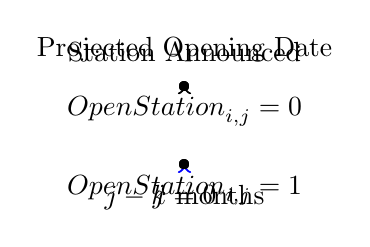
\begin{tikzpicture}
% Top arrow - Dashed
\node (A) at (\xmin,1) {};
\draw[dashed, ->, thick] (A) -- (\xmax,1);
\node (A1) at (\xmin,1) {\textbullet};
\node (A2) at (\xmid,1) {\textbullet};
% Bottom arrow - Dashed up to middle node, then solid
\node (B1) at (\xmin,0) {};
\node (B2) at (\xmid,0) {};
\draw[dashed, thick] (B1) -- (B2);  % Dashed part
\draw[->, thick, blue] (B2) -- (\xmax,0);     % Solid part
\node at (\xmin,0) {\textbullet};  % Left node bullet point
\node at (\xmid,0) {\textbullet};  % Middle node vertical line
% Labels for the bottom arrow nodes
\node[above] at (A1.north) {Station Announced};
\node[above] at (A2.north) {Projected Opening Date};
\node[below] at (B1.south) {$j-k$ months};
\node[below] at (B2.south) {$j=0$};
\node[below] at (\xmax,0) {$\text{Open Station}_{i,j}=1$};
\node[below] at (\xmax,1) {$\text{Open Station}_{i,j}=0$};
\end{tikzpicture}
\end{frame}
%%%%%%%%%%%%%%%%%%%%%%%%%%%%%%
\begin{frame}[noframenumbering,plain,allowframebreaks]{References}
    \printbibliography[heading=none]
\end{frame}
\end{document}
